% ------------------------------------------------------------------------
%DIF LATEXDIFF DIFFERENCE FILE
%DIF DEL proposta-oldtmp-28549.tex   Tue May 25 21:54:07 2021
%DIF ADD proposta.tex                Tue May 25 21:35:03 2021
% ------------------------------------------------------------------------
% Proposta inicial de projeto na disciplina de PI1A5
% Equipe TGT
% 1° semestre de 2021
% ------------------------------------------------------------------------
% ------------------------------------------------------------------------

\documentclass[
	% -- opções da classe memoir --
%DIF 11-19c11-14
%DIF < 	12pt,				% tamanho da fonte
%DIF < 	openright,			% capítulos começam em pág ímpar (insere página vazia caso preciso)
%DIF < 	oneside,			% twoside para impressão em verso e anverso. Oposto a oneside
%DIF < 	a4paper,			% tamanho do papel.
%DIF < 	% -- opções da classe abntex2 --
%DIF < 	%chapter=TITLE,		% títulos de capítulos convertidos em letras maiúsculas
%DIF < 	%section=TITLE,		% títulos de seções convertidos em letras maiúsculas
%DIF < 	%subsection=TITLE,	% títulos de subseções convertidos em letras maiúsculas
%DIF < 	%subsubsection=TITLE,% títulos de subsubseções convertidos em letras maiúsculas
%DIF -------
	12pt, %DIF > 
	openright, %DIF > 
	oneside, %DIF > 
	a4paper, %DIF > 
%DIF -------
	% -- opções do pacote babel --
%DIF 21-24c16-17
%DIF < 	english,			% idioma adicional para hifenização
%DIF < 	% french,				% idioma adicional para hifenização
%DIF < 	% spanish,			% idioma adicional para hifenização
%DIF < 	brazil				% o último idioma é o principal do documento
%DIF -------
	english, %DIF > 
	brazil %DIF > 
%DIF -------
]{abntex2}

%DIF 27-44c20-27
%DIF < % ---
%DIF < % Pacotes básicos
%DIF < % ---
%DIF < \usepackage{lmodern}			% Usa a fonte Latin Modern			
%DIF < \usepackage[T1]{fontenc}		% Selecao de codigos de fonte.
%DIF < \usepackage[utf8]{inputenc}		% Codificacao do documento (conversão automática dos acentos)
%DIF < \usepackage{lastpage}			% Usado pela Ficha catalográfica
%DIF < \usepackage{indentfirst}		% Indenta o primeiro parágrafo de cada seção.
%DIF < \usepackage{color}				% Controle das cores
%DIF < \usepackage{graphicx}			% Inclusão de gráficos
%DIF < \usepackage{microtype} 			% para melhorias de justificação
%DIF < % ---
%DIF < 
%DIF < % ---
%DIF < % Pacotes de citações
%DIF < % ---
%DIF < \usepackage[brazilian,hyperpageref]{backref}	 % Paginas com as citações na bibl
%DIF < \usepackage[alf]{abntex2cite}	% Citações padrão ABNT
%DIF -------
\usepackage{lmodern} %DIF > 
\usepackage[T1]{fontenc} %DIF > 
\usepackage[utf8]{inputenc} %DIF > 
\usepackage{lastpage} %DIF > 
\usepackage{indentfirst} %DIF > 
\usepackage{color} %DIF > 
\usepackage{graphicx} %DIF > 
\usepackage{microtype} %DIF > 
%DIF -------

%DIF 46-48c29-30
%DIF < % ---
%DIF < % CONFIGURAÇÕES DE PACOTES
%DIF < % ---
%DIF -------
\usepackage[brazilian,hyperpageref]{backref} %DIF > 
\usepackage[alf]{abntex2cite} %DIF > 
%DIF -------

%DIF 50-52d32
%DIF < % ---
%DIF < % Configurações do pacote backref
%DIF < % Usado sem a opção hyperpageref de backref
%DIF -------
\renewcommand{\backrefpagesname}{Citado na(s) página(s):~}
%DIF 54d33
%DIF < % Texto padrão antes do número das páginas
%DIF -------
\renewcommand{\backref}{}
%DIF 56d34
%DIF < % Define os textos da citação
%DIF -------
\renewcommand*{\backrefalt}[4]{
	\ifcase #1 %
		Nenhuma citação no texto.%
	\or
		Citado na página #2.%
	\else
		Citado #1 vezes nas páginas #2.%
	\fi}%
%DIF 65-70d42
%DIF < % ---
%DIF < 
%DIF < 
%DIF < 
%DIF < % Informações de dados para CAPA e FOLHA DE ROSTO
%DIF < %---
%DIF -------
% ---
\titulo{Aplicativo de Lista de Compras}
\autor{Alkindar José Ferraz Rodrigues \\ Carolina de Moraes Josephik \\ Fabio Mendes Torres \\ Gabriely de Jesus Santos Bicigo \\ Leonardo Naoki Narita}
\local{São Paulo\par}
\data{2021}
% \orientador{Lauro César Araujo}
% \coorientador{Equipe \abnTeX}
\instituicao{%
  Instituto Federal de Educação, Ciência e Tecnologia de São Paulo
  \par
  Campus São Paulo
  \par
  Tecnologia em Análise e Desenvolvimento de Sistemas}
\tipotrabalho{Tese (Doutorado)}
% O preambulo deve conter o tipo do trabalho, o objetivo,
% o nome da instituição e a área de concentração
\preambulo{Proposta inicial de projeto apresentada na disciplina de Projeto Integrado I no 1° semestre de 2021.\\
Prof. Ivan Francolin Martinez\\
Prof. José Braz de Araujo}
% --- 

% ---
% Adiciona o nome da instituição na capa
% ---
\renewcommand{\imprimircapa}{%
\begin{capa}%
\center
\ABNTEXchapterfont\ INSTITUTO FEDERAL DE EDUCAÇÃO, CIÊNCIA E TECNOLOGIA DE SÃO PAULO \par
CAMPUS SÃO PAULO \par
TECNOLOGIA EM ANÁLISE E DESENVOLVIMENTO DE SISTEMAS \par
\vspace*{1cm}
{\ABNTEXchapterfont\large\imprimirautor}
\vfill
\begin{center}
\ABNTEXchapterfont\bfseries\LARGE\imprimirtitulo
\end{center}
\vfill
\large\imprimirlocal
\large\imprimirdata
\vspace*{1cm}
\end{capa}
}
% ---

%DIF 73-77d44
%DIF < 
%DIF < % ---
%DIF < % Configurações de aparência do PDF final
%DIF < 
%DIF < % alterando o aspecto da cor azul
%DIF -------
\definecolor{blue}{RGB}{41,5,195}

%DIF 80d46
%DIF < % informações do PDF
%DIF -------
\makeatletter
\hypersetup{
%DIF 83d48
%DIF <      	%pagebackref=true,
%DIF -------
  pdftitle={\@title},
  pdfauthor={\@author},
  pdfsubject={\imprimirpreambulo},
  pdfcreator={LaTeX with abnTeX2},
  pdfkeywords={abnt}{latex}{abntex}{abntex2}{trabalho acadêmico},
%DIF 89-92c53-56
%DIF < 		colorlinks=true,       		% false: boxed links; true: colored links
%DIF <     	linkcolor=blue,          	% color of internal links
%DIF <     	citecolor=blue,        		% color of links to bibliography
%DIF <     	filecolor=magenta,      		% color of file links
%DIF -------
  colorlinks=true, %DIF > 
  linkcolor=blue, %DIF > 
  citecolor=blue, %DIF > 
  filecolor=magenta, %DIF > 
%DIF -------
  urlcolor=blue,
  bookmarksdepth=4
}
\makeatother
%DIF 97-101d61
%DIF < % ---
%DIF < 
%DIF < % ---
%DIF < % Espaçamentos entre linhas e parágrafos
%DIF < % ---
%DIF -------

%DIF 103d62
%DIF < % O tamanho do parágrafo é dado por:
%DIF -------
\setlength{\parindent}{1.3cm}
%DIF < 
%DIF -------
\setlength{\parskip}{0.2cm} %DIF > 
%DIF < % Controle do espaçamento entre um parágrafo e outro:
%DIF < \setlength{\parskip}{0.2cm}  % tente também \onelineskip
%DIF < 
%DIF < 
%DIF < 
%DIF < % ----
%DIF < % Início do documento
%DIF < % ----
%DIF PREAMBLE EXTENSION ADDED BY LATEXDIFF
%DIF UNDERLINE PREAMBLE %DIF PREAMBLE
\RequirePackage[normalem]{ulem} %DIF PREAMBLE
\RequirePackage{color}\definecolor{RED}{rgb}{1,0,0}\definecolor{BLUE}{rgb}{0,0,1} %DIF PREAMBLE
\providecommand{\DIFadd}[1]{{\protect\color{blue}\uwave{#1}}} %DIF PREAMBLE
\providecommand{\DIFdel}[1]{{\protect\color{red}\sout{#1}}}                      %DIF PREAMBLE
%DIF SAFE PREAMBLE %DIF PREAMBLE
\providecommand{\DIFaddbegin}{} %DIF PREAMBLE
\providecommand{\DIFaddend}{} %DIF PREAMBLE
\providecommand{\DIFdelbegin}{} %DIF PREAMBLE
\providecommand{\DIFdelend}{} %DIF PREAMBLE
%DIF FLOATSAFE PREAMBLE %DIF PREAMBLE
\providecommand{\DIFaddFL}[1]{\DIFadd{#1}} %DIF PREAMBLE
\providecommand{\DIFdelFL}[1]{\DIFdel{#1}} %DIF PREAMBLE
\providecommand{\DIFaddbeginFL}{} %DIF PREAMBLE
\providecommand{\DIFaddendFL}{} %DIF PREAMBLE
\providecommand{\DIFdelbeginFL}{} %DIF PREAMBLE
\providecommand{\DIFdelendFL}{} %DIF PREAMBLE
\newcommand{\DIFscaledelfig}{0.5}
%DIF HIGHLIGHTGRAPHICS PREAMBLE %DIF PREAMBLE
\RequirePackage{settobox} %DIF PREAMBLE
\RequirePackage{letltxmacro} %DIF PREAMBLE
\newsavebox{\DIFdelgraphicsbox} %DIF PREAMBLE
\newlength{\DIFdelgraphicswidth} %DIF PREAMBLE
\newlength{\DIFdelgraphicsheight} %DIF PREAMBLE
% store original definition of \includegraphics %DIF PREAMBLE
\LetLtxMacro{\DIFOincludegraphics}{\includegraphics} %DIF PREAMBLE
\newcommand{\DIFaddincludegraphics}[2][]{{\color{blue}\fbox{\DIFOincludegraphics[#1]{#2}}}} %DIF PREAMBLE
\newcommand{\DIFdelincludegraphics}[2][]{% %DIF PREAMBLE
\sbox{\DIFdelgraphicsbox}{\DIFOincludegraphics[#1]{#2}}% %DIF PREAMBLE
\settoboxwidth{\DIFdelgraphicswidth}{\DIFdelgraphicsbox} %DIF PREAMBLE
\settoboxtotalheight{\DIFdelgraphicsheight}{\DIFdelgraphicsbox} %DIF PREAMBLE
\scalebox{\DIFscaledelfig}{% %DIF PREAMBLE
\parbox[b]{\DIFdelgraphicswidth}{\usebox{\DIFdelgraphicsbox}\\[-\baselineskip] \rule{\DIFdelgraphicswidth}{0em}}\llap{\resizebox{\DIFdelgraphicswidth}{\DIFdelgraphicsheight}{% %DIF PREAMBLE
\setlength{\unitlength}{\DIFdelgraphicswidth}% %DIF PREAMBLE
\begin{picture}(1,1)% %DIF PREAMBLE
\thicklines\linethickness{2pt} %DIF PREAMBLE
{\color[rgb]{1,0,0}\put(0,0){\framebox(1,1){}}}% %DIF PREAMBLE
{\color[rgb]{1,0,0}\put(0,0){\line( 1,1){1}}}% %DIF PREAMBLE
{\color[rgb]{1,0,0}\put(0,1){\line(1,-1){1}}}% %DIF PREAMBLE
\end{picture}% %DIF PREAMBLE
}\hspace*{3pt}}} %DIF PREAMBLE
} %DIF PREAMBLE
\LetLtxMacro{\DIFOaddbegin}{\DIFaddbegin} %DIF PREAMBLE
\LetLtxMacro{\DIFOaddend}{\DIFaddend} %DIF PREAMBLE
\LetLtxMacro{\DIFOdelbegin}{\DIFdelbegin} %DIF PREAMBLE
\LetLtxMacro{\DIFOdelend}{\DIFdelend} %DIF PREAMBLE
\DeclareRobustCommand{\DIFaddbegin}{\DIFOaddbegin \let\includegraphics\DIFaddincludegraphics} %DIF PREAMBLE
\DeclareRobustCommand{\DIFaddend}{\DIFOaddend \let\includegraphics\DIFOincludegraphics} %DIF PREAMBLE
\DeclareRobustCommand{\DIFdelbegin}{\DIFOdelbegin \let\includegraphics\DIFdelincludegraphics} %DIF PREAMBLE
\DeclareRobustCommand{\DIFdelend}{\DIFOaddend \let\includegraphics\DIFOincludegraphics} %DIF PREAMBLE
\LetLtxMacro{\DIFOaddbeginFL}{\DIFaddbeginFL} %DIF PREAMBLE
\LetLtxMacro{\DIFOaddendFL}{\DIFaddendFL} %DIF PREAMBLE
\LetLtxMacro{\DIFOdelbeginFL}{\DIFdelbeginFL} %DIF PREAMBLE
\LetLtxMacro{\DIFOdelendFL}{\DIFdelendFL} %DIF PREAMBLE
\DeclareRobustCommand{\DIFaddbeginFL}{\DIFOaddbeginFL \let\includegraphics\DIFaddincludegraphics} %DIF PREAMBLE
\DeclareRobustCommand{\DIFaddendFL}{\DIFOaddendFL \let\includegraphics\DIFOincludegraphics} %DIF PREAMBLE
\DeclareRobustCommand{\DIFdelbeginFL}{\DIFOdelbeginFL \let\includegraphics\DIFdelincludegraphics} %DIF PREAMBLE
\DeclareRobustCommand{\DIFdelendFL}{\DIFOaddendFL \let\includegraphics\DIFOincludegraphics} %DIF PREAMBLE
%DIF END PREAMBLE EXTENSION ADDED BY LATEXDIFF

\begin{document}

%DIF <  Seleciona o idioma do documento (conforme pacotes do babel)
%DIF < \selectlanguage{english}
\selectlanguage{brazil}
\DIFdelbegin %DIFDELCMD < 

%DIFDELCMD < %%%
%DIF <  Retira espaço extra obsoleto entre as frases.
\DIFdelend \frenchspacing

%DIF <  ----------------------------------------------------------
%DIF <  ELEMENTOS PRÉ-TEXTUAIS
%DIF <  ----------------------------------------------------------
%DIF <  \pretextual
\DIFdelbegin %DIFDELCMD < 

%DIFDELCMD < %%%
%DIF <  ---
%DIF <  Capa
%DIF <  ---
\DIFdelend \imprimircapa
%DIF <  ---
\DIFdelbegin %DIFDELCMD < 

%DIFDELCMD < %%%
%DIF <  ---
%DIF <  Folha de rosto
%DIF <  (o * indica que haverá a ficha bibliográfica)
%DIF <  ---
\DIFdelend \imprimirfolhaderosto*
%DIF <  ---

%DIF <  ----------------------------------------------------------
%DIF <  ELEMENTOS TEXTUAIS
%DIF <  ----------------------------------------------------------
\textual

%DIF < -----------------------------------------------------------
%DIF <  CONTEÚDO
%DIF < -----------------------------------------------------------
\chapter{Introdução}

\section{Descrição do Problema}

Lorem ipsum dolor sia temet \cite[p. 3]{Kanan2015}.

\label{sec:objetivos}
\section{Objetivos}

O obetivo deste projeto é desenvolver um aplicativo multiplataforma,
focado no gerenciamento de listas de compras compartilhadas e que
apresente análises quanto à variação de preço para usuários
brasileiros. Para tal, é necessário que o aplicativo ofereça uma
interface intuitiva e responsiva, e que os sistemas back-end sejam
estáveis e rápidos.

Desta forma, uma arquitetura adequada seria uma aplicação em três
camadas, com um aplciativo front-end capaz de ser acessado tanto nos
dispositvos Android quanto iOS, e, eventualmente, web; que a api
disponível ao aplicativo seja bem estruturada conforme os padrões
REST; que os dados dos usúarios sejam armazenados de maneira segura e
criptografada; e que uma base dados volumosa seja fornececida de antemão para a
comodidade dos usuários quanto aos itens de mercado mais comuns no país.

\label{sec:solucao}
\section{Solução Proposta}

Tendo em vista o problema exposto e as limitações que serão levantadas
acerca dos concorrentes, propomos como solução o Aplicativo
\emph{Lixt}, que apresentará as seguintes funcionalidades, expostas em
ordem de dependências e nível de complexidade:

\begin{itemize}
\item Login\\
  O usuário deverá fazer login, de forma segura e privativa, para que
  possam acessar as funcionalidades que se seguem. Inicialmente, foi
  pensada uma solução na qual o login poderia ser opcional para as
  funcionalidades mais básicas, entretanto, isso impõe uma dificuldade
  na formulação de duas lógicas distintas no front-end.
\item Construir e gerenciar listas de compras\\
  O usário deverá ser capaz de criar e destruir listas de compras, adicionar ou
  remover itens de uma lista, especificar quantos itens devem ser
  comprados de cada produto e marcar itens como comprados. Esta
  funcionalidade é considerada a mais básica e essencial para a
  entrega do MVP.
\item Gerenciar categorias\\
  O usuário poderá atribuir categorias aos produtos adicionados,
  adicionar e deletar categorias, e filtrar itens de uma lista com base nelas.
\item Compartilhamento De Listas\\
  O usuário terá a possibilidade de compartilhar listas com outros
  usuários logados, e mudanças realizadas por um usário devem estar
  disponíveis para os outros usuários com acesso a lista.
\item Atribuição de itens para usuários em listas compartilhadas\\
  O usuário poderá atribuir, em listas compartilhadas, itens a pessoas
  com acesso a esta lista, como forma de direcionar quem deve comprar
  cada item.
\item Comentários em listas compartilhadas\\
  O usuário poderá adicionar, em um lista que tenha acesso,
  comentários associados a itens específicos com informações que
  considerar relevantes àquele produto, e estas notas devem estar
  disponíveis aos demais usuários que tenham acesso aquela lista
\item Gerenciamento de compras\\
  O usuário poderá realizar compras, vinculadas a uma lista e a um
  mercado, inserindo o preço pago por cada produto e, possivelmente,
  um desconto associado ao item. Quando o processo de for iniciado, o
  usuário verá o valor atualizado a ser pago no carrinho conforme os
  itens forem selecionados como ``pegos''.
\item Histórico de compras\\
  As compras realizadas deverão ser salvas e apresentadas conforme
  solicitadas pelo usuário, e apresentar o valor total em destaque, assim como a
  varição em relação as compras anteriores no mesmo mercado e com a
  mesma lista. Também, o preço de cada item deve apresentar a variação
  em relação ao valor anterior e posterior.
\item Análise estatística de compras\\
  Será apresentado ao usuário uma análise estatística dos itens
  comprados e dos valores pagos, em diversos níveis de
  especificidade. Planeja-se para a versão final do aplicativo que o
  usuário possa visulizar as seguintes variações:
  \begin{itemize}
  \item a variação de preço das diversas compras, levando em
    consideração ou não os mercados;
  \item quantas unidades de um item foi comprado por vez;
  \item a variação de preço do item a cada compra, levando os mercados
    em consideração;
  \item a variação de da média de preços de uma categoria,
    considerando ou não os mercados;
  \item a variação da média de preços de uma marca, considerando ou
    não os mercados.
  \end{itemize}
\end{itemize}

\section{Escopo do Projeto}
%%% Local Variables:
%%% mode: latex
%%% TeX-master: "../proposta"
%%% End:

%DIF <  PRIMEIRO CAPÍTULO

\chapter{Análise de Concorrentes}
Auditamos soluções que existem atualmente no mercado e, ao verificar as aplicações existentes, conclui-se que há intersecções nas funções dentre os aplicativos analisados. As funções mais básicas, como gerenciamento de itens e gerenciamento de listas, estão presentes em todos, tendo em vista que são essenciais em qualquer aplicativo de lista. Outras funções básicas que deveriam ser incluídas em qualquer aplicação de lista, como gerenciamento de categorias e compartilhamento de listas, não estão presentes em todos os aplicativos analisados.
Contudo, as divergências ficam claras quando analisamos o mecanismo das aplicações, entre elas destacam-se o Mealime e o Cozi Family Organizer que, apesar de serem voltados para as compras, cumprem também outras funcionalidades. O Mealime, cujo foco é o planejamento de refeições, e o Cozi Family Organizer, cujo foco é o planejamento familiar, deixam a desejar nas funções relacionadas às compras.
Entre os outros aplicativos analisados, é perceptível que não possuem todas as funcionalidades propostas nesse documento, principalmente quando se trata de compartilhamento de listas, uma vez que cada software lida de modo diferente diante dessa feature. O SoftList, por exemplo, permite o compartilhamento de lista, porém não é capaz de ser gerenciada por mais de um usuário, sendo apenas importada para o usuário no qual a lista está sendo compartilhada.
Ao analisar os aplicativos mais populares da categoria, constatamos que o Out Of Milk, Bring! e o OurGroceries, que são destaques na área, não se propõem a exibir análise estatística das compras do usuário e nem manter um histórico do que foi comprado.

\pagebreak

\section{Tabela de Comparação}

	\begin{figure}[h!]
	\centering
	%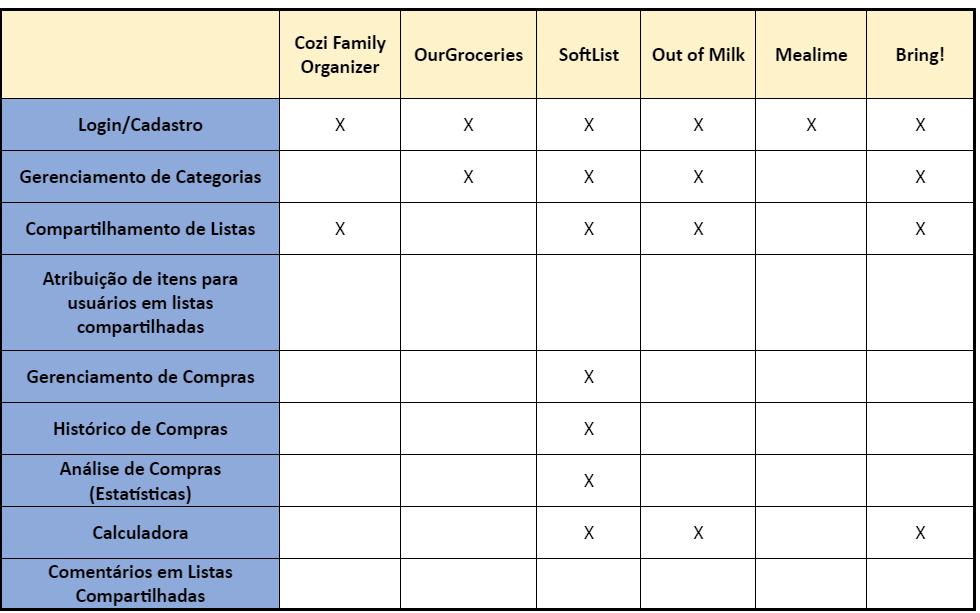
\includegraphics[scale=0.65]{./imagens/tabela_comparativa.png}
	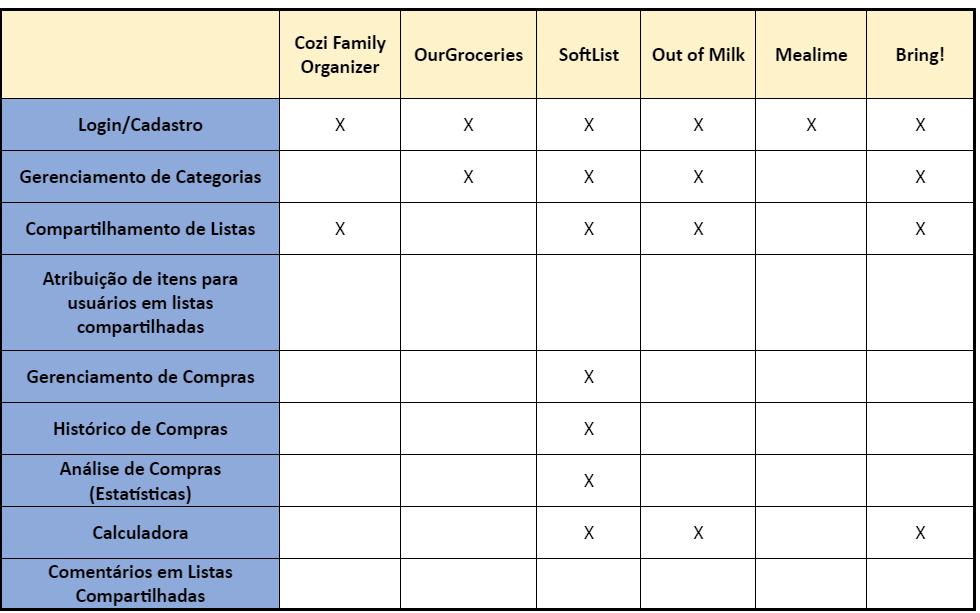
\includegraphics[width=.8\textwidth,height=\textheight,keepaspectratio]{./imagens/tabela_comparativa.png} 
	\caption{Comparativo de Concorrentes}
	\end{figure}
	

\chapter{Tecnologias Aplicadas}

\chapter{Gerenciamento do Projeto}
%DIF <  ÚLTIMO CAPÍTULO
%DIF < -----------------------------------------------------------

%DIF <  ----------------------------------------------------------
%DIF <  Finaliza a parte no bookmark do PDF
%DIF <  para que se inicie o bookmark na raiz
%DIF <  e adiciona espaço de parte no Sumário
%DIF <  ----------------------------------------------------------
\phantompart

%DIF <  ---
%DIF <  Conclusão
%DIF <  ---
%DIF < \include{capitulos/conclusao}
\DIFdelbegin %DIFDELCMD < 

%DIFDELCMD < %%%
%DIF <  ----------------------------------------------------------
%DIF <  ELEMENTOS PÓS-TEXTUAIS
%DIF <  ----------------------------------------------------------
\DIFdelend \postextual
%DIF <  ----------------------------------------------------------
\DIFdelbegin %DIFDELCMD < 

%DIFDELCMD < %%%
%DIF <  ----------------------------------------------------------
%DIF <  Referências bibliográficas
%DIF <  ----------------------------------------------------------
\DIFdelend \bibliography{referencias/referencias}

 %DIF <  ----------------------------------------------------------
%DIF <  Glossário
%DIF <  ----------------------------------------------------------
%DIF < 
%DIF <  Consulte o manual da classe abntex2 para orientações sobre o glossário.
%DIF < 
%DIF < \glossary
\DIFdelbegin %DIFDELCMD < 

%DIFDELCMD < %%%
%DIF <  ----------------------------------------------------------
%DIF <  Apêndices
%DIF <  ----------------------------------------------------------
%DIFDELCMD < 

%DIFDELCMD < %%%
%DIF <  ---
%DIF <  Inicia os apêndices
%DIF <  ---
%DIF < \include{capitulos/apendice}
%DIF <  ---
%DIFDELCMD < 

%DIFDELCMD < %%%
%DIF <  ----------------------------------------------------------
%DIF <  Anexos
%DIF <  ----------------------------------------------------------
%DIFDELCMD < 

%DIFDELCMD < %%%
%DIF <  ---
%DIF <  Inicia os anexos
%DIF <  ---
%DIF < \include{capitulos/anexo}
%DIFDELCMD < 

%DIFDELCMD < %%%
%DIF <  Fim do documento
 \DIFdelend\end{document}

%%% Local Variables:
%%% mode: latex
%%% TeX-master: t
%%% End:
